\documentclass[1p]{elsarticle_modified}
%\bibliographystyle{elsarticle-num}

%\usepackage[colorlinks]{hyperref}
%\usepackage{abbrmath_seonhwa} %\Abb, \Ascr, \Acal ,\Abf, \Afrak
\usepackage{amsfonts}
\usepackage{amssymb}
\usepackage{amsmath}
\usepackage{amsthm}
\usepackage{scalefnt}
\usepackage{amsbsy}
\usepackage{kotex}
\usepackage{caption}
\usepackage{subfig}
\usepackage{color}
\usepackage{graphicx}
\usepackage{xcolor} %% white, black, red, green, blue, cyan, magenta, yellow
\usepackage{float}
\usepackage{setspace}
\usepackage{hyperref}

\usepackage{tikz}
\usetikzlibrary{arrows}

\usepackage{multirow}
\usepackage{array} % fixed length table
\usepackage{hhline}

%%%%%%%%%%%%%%%%%%%%%
\makeatletter
\renewcommand*\env@matrix[1][\arraystretch]{%
	\edef\arraystretch{#1}%
	\hskip -\arraycolsep
	\let\@ifnextchar\new@ifnextchar
	\array{*\c@MaxMatrixCols c}}
\makeatother %https://tex.stackexchange.com/questions/14071/how-can-i-increase-the-line-spacing-in-a-matrix
%%%%%%%%%%%%%%%

\usepackage[normalem]{ulem}

\newcommand{\msout}[1]{\ifmmode\text{\sout{\ensuremath{#1}}}\else\sout{#1}\fi}
%SOURCE: \msout is \stkout macro in https://tex.stackexchange.com/questions/20609/strikeout-in-math-mode

\newcommand{\cancel}[1]{
	\ifmmode
	{\color{red}\msout{#1}}
	\else
	{\color{red}\sout{#1}}
	\fi
}

\newcommand{\add}[1]{
	{\color{blue}\uwave{#1}}
}

\newcommand{\replace}[2]{
	\ifmmode
	{\color{red}\msout{#1}}{\color{blue}\uwave{#2}}
	\else
	{\color{red}\sout{#1}}{\color{blue}\uwave{#2}}
	\fi
}

\newcommand{\Sol}{\mathcal{S}} %segment
\newcommand{\D}{D} %diagram
\newcommand{\A}{\mathcal{A}} %arc


%%%%%%%%%%%%%%%%%%%%%%%%%%%%%5 test

\def\sl{\operatorname{\textup{SL}}(2,\Cbb)}
\def\psl{\operatorname{\textup{PSL}}(2,\Cbb)}
\def\quan{\mkern 1mu \triangleright \mkern 1mu}

\theoremstyle{definition}
\newtheorem{thm}{Theorem}[section]
\newtheorem{prop}[thm]{Proposition}
\newtheorem{lem}[thm]{Lemma}
\newtheorem{ques}[thm]{Question}
\newtheorem{cor}[thm]{Corollary}
\newtheorem{defn}[thm]{Definition}
\newtheorem{exam}[thm]{Example}
\newtheorem{rmk}[thm]{Remark}
\newtheorem{alg}[thm]{Algorithm}

\newcommand{\I}{\sqrt{-1}}
\begin{document}

%\begin{frontmatter}
%
%\title{Boundary parabolic representations of knots up to 8 crossings}
%
%%% Group authors per affiliation:
%\author{Yunhi Cho} 
%\address{Department of Mathematics, University of Seoul, Seoul, Korea}
%\ead{yhcho@uos.ac.kr}
%
%
%\author{Seonhwa Kim} %\fnref{s_kim}}
%\address{Center for Geometry and Physics, Institute for Basic Science, Pohang, 37673, Korea}
%\ead{ryeona17@ibs.re.kr}
%
%\author{Hyuk Kim}
%\address{Department of Mathematical Sciences, Seoul National University, Seoul 08826, Korea}
%\ead{hyukkim@snu.ac.kr}
%
%\author{Seokbeom Yoon}
%\address{Department of Mathematical Sciences, Seoul National University, Seoul, 08826,  Korea}
%\ead{sbyoon15@snu.ac.kr}
%
%\begin{abstract}
%We find all boundary parabolic representation of knots up to 8 crossings.
%
%\end{abstract}
%\begin{keyword}
%    \MSC[2010] 57M25 
%\end{keyword}
%
%\end{frontmatter}

%\linenumbers
%\tableofcontents
%
\newcommand\colored[1]{\textcolor{white}{\rule[-0.35ex]{0.8em}{1.4ex}}\kern-0.8em\color{red} #1}%
%\newcommand\colored[1]{\textcolor{white}{ #1}\kern-2.17ex	\textcolor{white}{ #1}\kern-1.81ex	\textcolor{white}{ #1}\kern-2.15ex\color{red}#1	}

{\Large $\underline{12n_{0821}~(K12n_{0821})}$}

\setlength{\tabcolsep}{10pt}
\renewcommand{\arraystretch}{1.6}
\vspace{1cm}\begin{tabular}{m{100pt}>{\centering\arraybackslash}m{274pt}}
\multirow{5}{120pt}{
	\centering
	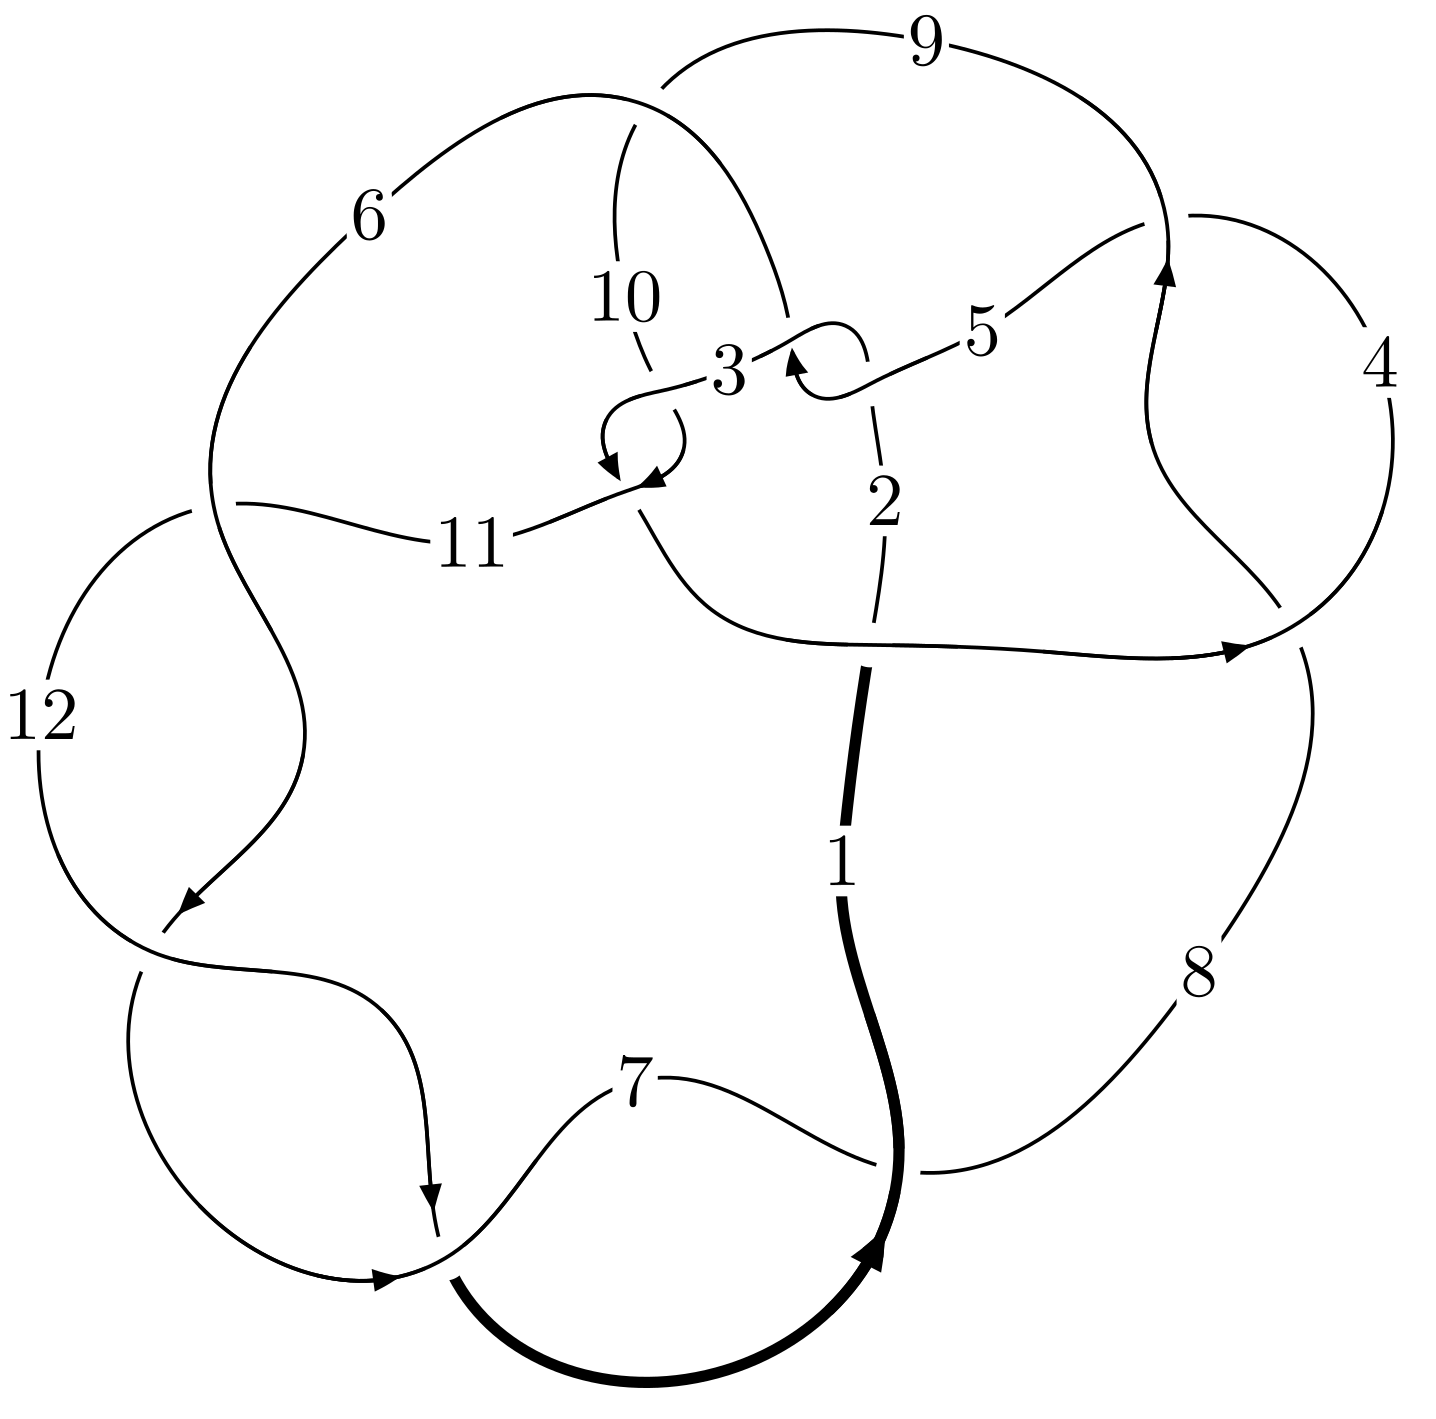
\includegraphics[width=112pt]{../../../GIT/diagram.site/Diagrams/png/2910_12n_0821.png}\\
\ \ \ A knot diagram\footnotemark}&
\allowdisplaybreaks
\textbf{Linearized knot diagam} \\
\cline{2-2}
 &
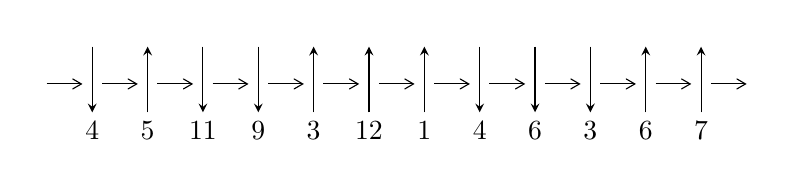
\begin{tikzpicture}[x=20pt, y=17pt]
	% nodes
	\node (C0) at (0, 0) {};
	\node (C1) at (1, 0) {};
	\node (C1U) at (1, +1) {};
	\node (C1D) at (1, -1) {4};

	\node (C2) at (2, 0) {};
	\node (C2U) at (2, +1) {};
	\node (C2D) at (2, -1) {5};

	\node (C3) at (3, 0) {};
	\node (C3U) at (3, +1) {};
	\node (C3D) at (3, -1) {11};

	\node (C4) at (4, 0) {};
	\node (C4U) at (4, +1) {};
	\node (C4D) at (4, -1) {9};

	\node (C5) at (5, 0) {};
	\node (C5U) at (5, +1) {};
	\node (C5D) at (5, -1) {3};

	\node (C6) at (6, 0) {};
	\node (C6U) at (6, +1) {};
	\node (C6D) at (6, -1) {12};

	\node (C7) at (7, 0) {};
	\node (C7U) at (7, +1) {};
	\node (C7D) at (7, -1) {1};

	\node (C8) at (8, 0) {};
	\node (C8U) at (8, +1) {};
	\node (C8D) at (8, -1) {4};

	\node (C9) at (9, 0) {};
	\node (C9U) at (9, +1) {};
	\node (C9D) at (9, -1) {6};

	\node (C10) at (10, 0) {};
	\node (C10U) at (10, +1) {};
	\node (C10D) at (10, -1) {3};

	\node (C11) at (11, 0) {};
	\node (C11U) at (11, +1) {};
	\node (C11D) at (11, -1) {6};

	\node (C12) at (12, 0) {};
	\node (C12U) at (12, +1) {};
	\node (C12D) at (12, -1) {7};
	\node (C13) at (13, 0) {};

	% arrows
	\draw[->,>={angle 60}]
	(C0) edge (C1) (C1) edge (C2) (C2) edge (C3) (C3) edge (C4) (C4) edge (C5) (C5) edge (C6) (C6) edge (C7) (C7) edge (C8) (C8) edge (C9) (C9) edge (C10) (C10) edge (C11) (C11) edge (C12) (C12) edge (C13) ;	\draw[->,>=stealth]
	(C1U) edge (C1D) (C2D) edge (C2U) (C3U) edge (C3D) (C4U) edge (C4D) (C5D) edge (C5U) (C6D) edge (C6U) (C7D) edge (C7U) (C8U) edge (C8D) (C9U) edge (C9D) (C10U) edge (C10D) (C11D) edge (C11U) (C12D) edge (C12U) ;
	\end{tikzpicture} \\
\hhline{~~} \\& 
\textbf{Solving Sequence} \\ \cline{2-2} 
 &
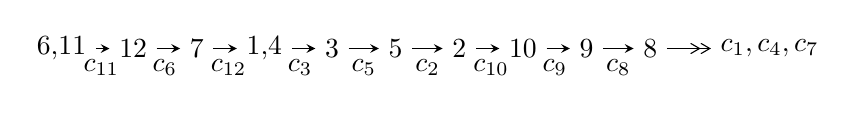
\begin{tikzpicture}[x=23pt, y=7pt]
	% node
	\node (A0) at (-1/8, 0) {6,11};
	\node (A1) at (1, 0) {12};
	\node (A2) at (2, 0) {7};
	\node (A3) at (49/16, 0) {1,4};
	\node (A4) at (33/8, 0) {3};
	\node (A5) at (41/8, 0) {5};
	\node (A6) at (49/8, 0) {2};
	\node (A7) at (57/8, 0) {10};
	\node (A8) at (65/8, 0) {9};
	\node (A9) at (73/8, 0) {8};
	\node (C1) at (1/2, -1) {$c_{11}$};
	\node (C2) at (3/2, -1) {$c_{6}$};
	\node (C3) at (5/2, -1) {$c_{12}$};
	\node (C4) at (29/8, -1) {$c_{3}$};
	\node (C5) at (37/8, -1) {$c_{5}$};
	\node (C6) at (45/8, -1) {$c_{2}$};
	\node (C7) at (53/8, -1) {$c_{10}$};
	\node (C8) at (61/8, -1) {$c_{9}$};
	\node (C9) at (69/8, -1) {$c_{8}$};
	\node (A10) at (11, 0) {$c_{1},c_{4},c_{7}$};

	% edge
	\draw[->,>=stealth]	
	(A0) edge (A1) (A1) edge (A2) (A2) edge (A3) (A3) edge (A4) (A4) edge (A5) (A5) edge (A6) (A6) edge (A7) (A7) edge (A8) (A8) edge (A9) ;
	\draw[->>,>={angle 60}]	
	(A9) edge (A10);
\end{tikzpicture} \\ 

\end{tabular} \\

\footnotetext{
The image of knot diagram is generated by the software ``\textbf{Draw programme}" developed by Andrew Bartholomew(\url{http://www.layer8.co.uk/maths/draw/index.htm\#Running-draw}), where we modified some parts for our purpose(\url{https://github.com/CATsTAILs/LinksPainter}).
}\phantom \\ \newline 
\centering \textbf{Ideals for irreducible components\footnotemark of $X_{\text{par}}$} 
 
\begin{align*}
I^u_{1}&=\langle 
5 u^{12}+17 u^{11}-8 u^{10}-70 u^9-18 u^8+113 u^7+91 u^6-46 u^5-122 u^4-31 u^3+55 u^2+2 b+23 u+12,\\
\phantom{I^u_{1}}&\phantom{= \langle  }-11 u^{12}-36 u^{11}+\cdots+2 a-27,\\
\phantom{I^u_{1}}&\phantom{= \langle  }u^{13}+5 u^{12}+4 u^{11}-16 u^{10}-26 u^9+15 u^8+53 u^7+22 u^6-36 u^5-45 u^4- u^3+21 u^2+10 u+4\rangle \\
I^u_{2}&=\langle 
- u^7+5 u^5- u^4-7 u^3+3 u^2+b+2 u-1,\;u^7-5 u^5+u^4+7 u^3-4 u^2+a-2 u+3,\\
\phantom{I^u_{2}}&\phantom{= \langle  }u^8-6 u^6+u^5+11 u^4-4 u^3-6 u^2+3 u+1\rangle \\
I^u_{3}&=\langle 
- a^3 u^2-10 a^3 u+2 a^2 u^2+8 a^3-9 a^2 u+16 u^2 a+13 a^2-14 a u+19 u^2+29 b-12 a-13 u-36,\\
\phantom{I^u_{3}}&\phantom{= \langle  }-2 a^3 u^2+a^4+a^3 u+3 a^2 u^2+4 a^3- a^2 u+12 u^2 a-5 a^2-7 a u-27 a+u+1,\;u^3- u^2-2 u+1\rangle \\
\\
\end{align*}
\raggedright * 3 irreducible components of $\dim_{\mathbb{C}}=0$, with total 33 representations.\\
\footnotetext{All coefficients of polynomials are rational numbers. But the coefficients are sometimes approximated in decimal forms when there is not enough margin.}
\newpage
\renewcommand{\arraystretch}{1}
\centering \section*{I. $I^u_{1}= \langle 5 u^{12}+17 u^{11}+\cdots+2 b+12,\;-11 u^{12}-36 u^{11}+\cdots+2 a-27,\;u^{13}+5 u^{12}+\cdots+10 u+4 \rangle$}
\flushleft \textbf{(i) Arc colorings}\\
\begin{tabular}{m{7pt} m{180pt} m{7pt} m{180pt} }
\flushright $a_{6}=$&$\begin{pmatrix}0\\u\end{pmatrix}$ \\
\flushright $a_{11}=$&$\begin{pmatrix}1\\0\end{pmatrix}$ \\
\flushright $a_{12}=$&$\begin{pmatrix}1\\- u^2\end{pmatrix}$ \\
\flushright $a_{7}=$&$\begin{pmatrix}u\\- u^3+u\end{pmatrix}$ \\
\flushright $a_{1}=$&$\begin{pmatrix}- u^2+1\\u^4-2 u^2\end{pmatrix}$ \\
\flushright $a_{4}=$&$\begin{pmatrix}\frac{11}{2} u^{12}+18 u^{11}+\cdots+24 u+\frac{27}{2}\\-\frac{5}{2} u^{12}-\frac{17}{2} u^{11}+\cdots-\frac{23}{2} u-6\end{pmatrix}$ \\
\flushright $a_{3}=$&$\begin{pmatrix}3 u^{12}+\frac{19}{2} u^{11}+\cdots+\frac{25}{2} u+\frac{15}{2}\\-\frac{5}{2} u^{12}-\frac{17}{2} u^{11}+\cdots-\frac{23}{2} u-6\end{pmatrix}$ \\
\flushright $a_{5}=$&$\begin{pmatrix}\frac{11}{4} u^{12}+\frac{37}{4} u^{11}+\cdots+\frac{49}{4} u+7\\-\frac{1}{2} u^{12}-\frac{3}{2} u^{11}+\cdots-\frac{3}{2} u-1\end{pmatrix}$ \\
\flushright $a_{2}=$&$\begin{pmatrix}-\frac{11}{4} u^{12}-\frac{37}{4} u^{11}+\cdots-\frac{53}{4} u-6\\-\frac{1}{2} u^{12}-\frac{3}{2} u^{11}+\cdots-\frac{3}{2} u-1\end{pmatrix}$ \\
\flushright $a_{10}=$&$\begin{pmatrix}\frac{1}{4} u^{12}+\frac{3}{4} u^{11}+\cdots-\frac{1}{4} u+1\\\frac{1}{2} u^{12}+\frac{3}{2} u^{11}+\cdots+\frac{3}{2} u+1\end{pmatrix}$ \\
\flushright $a_{9}=$&$\begin{pmatrix}\frac{1}{4} u^{12}+\frac{3}{4} u^{11}+\cdots-\frac{1}{4} u+1\\-\frac{1}{2} u^{12}-\frac{3}{2} u^{11}+\cdots-\frac{5}{2} u-1\end{pmatrix}$ \\
\flushright $a_{8}=$&$\begin{pmatrix}u^3-2 u\\- u^5+3 u^3- u\end{pmatrix}$\\&\end{tabular}
\flushleft \textbf{(ii) Obstruction class $= -1$}\\~\\
\flushleft \textbf{(iii) Cusp Shapes $= -17 u^{12}-55 u^{11}+30 u^{10}+220 u^9+44 u^8-346 u^7-267 u^6+135 u^5+358 u^4+81 u^3-157 u^2-56 u-34$}\\~\\
\newpage\renewcommand{\arraystretch}{1}
\flushleft \textbf{(iv) u-Polynomials at the component}\newline \\
\begin{tabular}{m{50pt}|m{274pt}}
Crossings & \hspace{64pt}u-Polynomials at each crossing \\
\hline $$\begin{aligned}c_{1}\end{aligned}$$&$\begin{aligned}
&u^{13}- u^{12}+\cdots+15 u+1
\end{aligned}$\\
\hline $$\begin{aligned}c_{2},c_{5}\end{aligned}$$&$\begin{aligned}
&u^{13}+6 u^{12}+\cdots+12 u+8
\end{aligned}$\\
\hline $$\begin{aligned}c_{3},c_{4},c_{8}\\c_{10}\end{aligned}$$&$\begin{aligned}
&u^{13}- u^{12}+\cdots+u-1
\end{aligned}$\\
\hline $$\begin{aligned}c_{6},c_{7},c_{11}\\c_{12}\end{aligned}$$&$\begin{aligned}
&u^{13}-5 u^{12}+\cdots+10 u-4
\end{aligned}$\\
\hline $$\begin{aligned}c_{9}\end{aligned}$$&$\begin{aligned}
&u^{13}+15 u^{11}+\cdots-15 u^2-1
\end{aligned}$\\
\hline
\end{tabular}\\~\\
\newpage\renewcommand{\arraystretch}{1}
\flushleft \textbf{(v) Riley Polynomials at the component}\newline \\
\begin{tabular}{m{50pt}|m{274pt}}
Crossings & \hspace{64pt}Riley Polynomials at each crossing \\
\hline $$\begin{aligned}c_{1}\end{aligned}$$&$\begin{aligned}
&y^{13}+39 y^{12}+\cdots+155 y-1
\end{aligned}$\\
\hline $$\begin{aligned}c_{2},c_{5}\end{aligned}$$&$\begin{aligned}
&y^{13}-14 y^{12}+\cdots+80 y-64
\end{aligned}$\\
\hline $$\begin{aligned}c_{3},c_{4},c_{8}\\c_{10}\end{aligned}$$&$\begin{aligned}
&y^{13}+7 y^{12}+\cdots- y-1
\end{aligned}$\\
\hline $$\begin{aligned}c_{6},c_{7},c_{11}\\c_{12}\end{aligned}$$&$\begin{aligned}
&y^{13}-17 y^{12}+\cdots-68 y-16
\end{aligned}$\\
\hline $$\begin{aligned}c_{9}\end{aligned}$$&$\begin{aligned}
&y^{13}+30 y^{12}+\cdots-30 y-1
\end{aligned}$\\
\hline
\end{tabular}\\~\\
\newpage\flushleft \textbf{(vi) Complex Volumes and Cusp Shapes}
$$\begin{array}{c|c|c}  
\text{Solutions to }I^u_{1}& \I (\text{vol} + \sqrt{-1}CS) & \text{Cusp shape}\\
 \hline 
\begin{aligned}
u &= -0.497615 + 0.876393 I \\
a &= -0.520432 - 0.143375 I \\
b &= -0.286884 - 1.048300 I\end{aligned}
 & \phantom{-}5.56724 - 2.86079 I & \phantom{-}6.58762 + 4.73580 I \\ \hline\begin{aligned}
u &= -0.497615 - 0.876393 I \\
a &= -0.520432 + 0.143375 I \\
b &= -0.286884 + 1.048300 I\end{aligned}
 & \phantom{-}5.56724 + 2.86079 I & \phantom{-}6.58762 - 4.73580 I \\ \hline\begin{aligned}
u &= \phantom{-}0.977918 + 0.258584 I \\
a &= -0.50072 - 1.42125 I \\
b &= -0.432880 + 0.770070 I\end{aligned}
 & \phantom{-}3.49671 + 3.30133 I & \phantom{-}5.66986 - 7.29619 I \\ \hline\begin{aligned}
u &= \phantom{-}0.977918 - 0.258584 I \\
a &= -0.50072 + 1.42125 I \\
b &= -0.432880 - 0.770070 I\end{aligned}
 & \phantom{-}3.49671 - 3.30133 I & \phantom{-}5.66986 + 7.29619 I \\ \hline\begin{aligned}
u &= -1.15240\phantom{ +0.000000I} \\
a &= -0.0663024\phantom{ +0.000000I} \\
b &= -0.413299\phantom{ +0.000000I}\end{aligned}
 & \phantom{-}2.44636\phantom{ +0.000000I} & \phantom{-}4.36790\phantom{ +0.000000I} \\ \hline\begin{aligned}
u &= \phantom{-}1.276260 + 0.459752 I \\
a &= \phantom{-}0.350061 + 1.031200 I \\
b &= \phantom{-}0.82833 - 1.24672 I\end{aligned}
 & \phantom{-}11.16010 + 7.44705 I & \phantom{-}5.81652 - 5.20775 I \\ \hline\begin{aligned}
u &= \phantom{-}1.276260 - 0.459752 I \\
a &= \phantom{-}0.350061 - 1.031200 I \\
b &= \phantom{-}0.82833 + 1.24672 I\end{aligned}
 & \phantom{-}11.16010 - 7.44705 I & \phantom{-}5.81652 + 5.20775 I \\ \hline\begin{aligned}
u &= -0.158213 + 0.403429 I \\
a &= \phantom{-}0.826836 - 0.260199 I \\
b &= \phantom{-}0.295622 + 0.443698 I\end{aligned}
 & -0.016018 - 0.973727 I & -0.21220 + 6.98709 I \\ \hline\begin{aligned}
u &= -0.158213 - 0.403429 I \\
a &= \phantom{-}0.826836 + 0.260199 I \\
b &= \phantom{-}0.295622 - 0.443698 I\end{aligned}
 & -0.016018 + 0.973727 I & -0.21220 - 6.98709 I \\ \hline\begin{aligned}
u &= -1.71570 + 0.06763 I \\
a &= \phantom{-}0.12881 - 1.62879 I \\
b &= \phantom{-}0.519770 + 0.949390 I\end{aligned}
 & \phantom{-}13.07970 - 4.61256 I & \phantom{-}6.03428 + 7.03944 I\\
 \hline 
 \end{array}$$\newpage$$\begin{array}{c|c|c}  
\text{Solutions to }I^u_{1}& \I (\text{vol} + \sqrt{-1}CS) & \text{Cusp shape}\\
 \hline 
\begin{aligned}
u &= -1.71570 - 0.06763 I \\
a &= \phantom{-}0.12881 + 1.62879 I \\
b &= \phantom{-}0.519770 - 0.949390 I\end{aligned}
 & \phantom{-}13.07970 + 4.61256 I & \phantom{-}6.03428 - 7.03944 I \\ \hline\begin{aligned}
u &= -1.80645 + 0.12280 I \\
a &= \phantom{-}0.24859 + 1.52769 I \\
b &= -1.21731 - 1.42694 I\end{aligned}
 & -17.2391 - 10.0928 I & \phantom{-}5.92000 + 4.03274 I \\ \hline\begin{aligned}
u &= -1.80645 - 0.12280 I \\
a &= \phantom{-}0.24859 - 1.52769 I \\
b &= -1.21731 + 1.42694 I\end{aligned}
 & -17.2391 + 10.0928 I & \phantom{-}5.92000 - 4.03274 I\\
 \hline 
 \end{array}$$\newpage\newpage\renewcommand{\arraystretch}{1}
\centering \section*{II. $I^u_{2}= \langle - u^7+5 u^5- u^4-7 u^3+3 u^2+b+2 u-1,\;u^7-5 u^5+u^4+7 u^3-4 u^2+a-2 u+3,\;u^8-6 u^6+u^5+11 u^4-4 u^3-6 u^2+3 u+1 \rangle$}
\flushleft \textbf{(i) Arc colorings}\\
\begin{tabular}{m{7pt} m{180pt} m{7pt} m{180pt} }
\flushright $a_{6}=$&$\begin{pmatrix}0\\u\end{pmatrix}$ \\
\flushright $a_{11}=$&$\begin{pmatrix}1\\0\end{pmatrix}$ \\
\flushright $a_{12}=$&$\begin{pmatrix}1\\- u^2\end{pmatrix}$ \\
\flushright $a_{7}=$&$\begin{pmatrix}u\\- u^3+u\end{pmatrix}$ \\
\flushright $a_{1}=$&$\begin{pmatrix}- u^2+1\\u^4-2 u^2\end{pmatrix}$ \\
\flushright $a_{4}=$&$\begin{pmatrix}- u^7+5 u^5- u^4-7 u^3+4 u^2+2 u-3\\u^7-5 u^5+u^4+7 u^3-3 u^2-2 u+1\end{pmatrix}$ \\
\flushright $a_{3}=$&$\begin{pmatrix}u^2-2\\u^7-5 u^5+u^4+7 u^3-3 u^2-2 u+1\end{pmatrix}$ \\
\flushright $a_{5}=$&$\begin{pmatrix}- u^5+4 u^3-4 u\\- u^4+3 u^2-1\end{pmatrix}$ \\
\flushright $a_{2}=$&$\begin{pmatrix}u^5- u^4-4 u^3+3 u^2+3 u-1\\u^4-3 u^2+1\end{pmatrix}$ \\
\flushright $a_{10}=$&$\begin{pmatrix}u^7-6 u^5+u^4+10 u^3-4 u^2-3 u+3\\- u^3+2 u-1\end{pmatrix}$ \\
\flushright $a_{9}=$&$\begin{pmatrix}u^7-6 u^5+u^4+10 u^3-4 u^2-3 u+3\\u^5-4 u^3+3 u-1\end{pmatrix}$ \\
\flushright $a_{8}=$&$\begin{pmatrix}- u^3+2 u\\u^5-3 u^3+u\end{pmatrix}$\\&\end{tabular}
\flushleft \textbf{(ii) Obstruction class $= 1$}\\~\\
\flushleft \textbf{(iii) Cusp Shapes $= -3 u^7+2 u^6+21 u^5-12 u^4-42 u^3+24 u^2+17 u-10$}\\~\\
\newpage\renewcommand{\arraystretch}{1}
\flushleft \textbf{(iv) u-Polynomials at the component}\newline \\
\begin{tabular}{m{50pt}|m{274pt}}
Crossings & \hspace{64pt}u-Polynomials at each crossing \\
\hline $$\begin{aligned}c_{1}\end{aligned}$$&$\begin{aligned}
&u^8+3 u^7+6 u^6+4 u^5-7 u^4-12 u^3- u^2+6 u+1
\end{aligned}$\\
\hline $$\begin{aligned}c_{2}\end{aligned}$$&$\begin{aligned}
&u^8+3 u^7- u^6-11 u^5-6 u^4+11 u^3+8 u^2-3 u-1
\end{aligned}$\\
\hline $$\begin{aligned}c_{3},c_{8}\end{aligned}$$&$\begin{aligned}
&u^8+u^7-2 u^6-2 u^5- u^4+u^2+1
\end{aligned}$\\
\hline $$\begin{aligned}c_{4},c_{10}\end{aligned}$$&$\begin{aligned}
&u^8- u^7-2 u^6+2 u^5- u^4+u^2+1
\end{aligned}$\\
\hline $$\begin{aligned}c_{5}\end{aligned}$$&$\begin{aligned}
&u^8-3 u^7- u^6+11 u^5-6 u^4-11 u^3+8 u^2+3 u-1
\end{aligned}$\\
\hline $$\begin{aligned}c_{6},c_{7}\end{aligned}$$&$\begin{aligned}
&u^8-6 u^6- u^5+11 u^4+4 u^3-6 u^2-3 u+1
\end{aligned}$\\
\hline $$\begin{aligned}c_{9}\end{aligned}$$&$\begin{aligned}
&u^8+u^6- u^4-2 u^3-2 u^2+u+1
\end{aligned}$\\
\hline $$\begin{aligned}c_{11},c_{12}\end{aligned}$$&$\begin{aligned}
&u^8-6 u^6+u^5+11 u^4-4 u^3-6 u^2+3 u+1
\end{aligned}$\\
\hline
\end{tabular}\\~\\
\newpage\renewcommand{\arraystretch}{1}
\flushleft \textbf{(v) Riley Polynomials at the component}\newline \\
\begin{tabular}{m{50pt}|m{274pt}}
Crossings & \hspace{64pt}Riley Polynomials at each crossing \\
\hline $$\begin{aligned}c_{1}\end{aligned}$$&$\begin{aligned}
&y^8+3 y^7-2 y^6-30 y^5+99 y^4-166 y^3+131 y^2-38 y+1
\end{aligned}$\\
\hline $$\begin{aligned}c_{2},c_{5}\end{aligned}$$&$\begin{aligned}
&y^8-11 y^7+55 y^6-159 y^5+278 y^4-281 y^3+142 y^2-25 y+1
\end{aligned}$\\
\hline $$\begin{aligned}c_{3},c_{4},c_{8}\\c_{10}\end{aligned}$$&$\begin{aligned}
&y^8-5 y^7+6 y^6+2 y^5- y^4-6 y^3- y^2+2 y+1
\end{aligned}$\\
\hline $$\begin{aligned}c_{6},c_{7},c_{11}\\c_{12}\end{aligned}$$&$\begin{aligned}
&y^8-12 y^7+58 y^6-145 y^5+203 y^4-166 y^3+82 y^2-21 y+1
\end{aligned}$\\
\hline $$\begin{aligned}c_{9}\end{aligned}$$&$\begin{aligned}
&y^8+2 y^7- y^6-6 y^5- y^4+2 y^3+6 y^2-5 y+1
\end{aligned}$\\
\hline
\end{tabular}\\~\\
\newpage\flushleft \textbf{(vi) Complex Volumes and Cusp Shapes}
$$\begin{array}{c|c|c}  
\text{Solutions to }I^u_{2}& \I (\text{vol} + \sqrt{-1}CS) & \text{Cusp shape}\\
 \hline 
\begin{aligned}
u &= -0.868162\phantom{ +0.000000I} \\
a &= \phantom{-}0.196614\phantom{ +0.000000I} \\
b &= -1.44291\phantom{ +0.000000I}\end{aligned}
 & -1.71749\phantom{ +0.000000I} & \phantom{-}5.61020\phantom{ +0.000000I} \\ \hline\begin{aligned}
u &= \phantom{-}0.733070 + 0.412657 I \\
a &= -1.46575 - 0.08392 I \\
b &= -0.167149 + 0.688931 I\end{aligned}
 & \phantom{-}4.59844 + 1.46844 I & \phantom{-}5.92040 - 3.51787 I \\ \hline\begin{aligned}
u &= \phantom{-}0.733070 - 0.412657 I \\
a &= -1.46575 + 0.08392 I \\
b &= -0.167149 - 0.688931 I\end{aligned}
 & \phantom{-}4.59844 - 1.46844 I & \phantom{-}5.92040 + 3.51787 I \\ \hline\begin{aligned}
u &= \phantom{-}1.35093\phantom{ +0.000000I} \\
a &= \phantom{-}0.698866\phantom{ +0.000000I} \\
b &= -0.873848\phantom{ +0.000000I}\end{aligned}
 & \phantom{-}1.54653\phantom{ +0.000000I} & -4.73980\phantom{ +0.000000I} \\ \hline\begin{aligned}
u &= \phantom{-}1.69498\phantom{ +0.000000I} \\
a &= -0.701727\phantom{ +0.000000I} \\
b &= \phantom{-}1.57470\phantom{ +0.000000I}\end{aligned}
 & \phantom{-}7.46249\phantom{ +0.000000I} & \phantom{-}4.83590\phantom{ +0.000000I} \\ \hline\begin{aligned}
u &= -1.69932 + 0.10356 I \\
a &= \phantom{-}0.446197 - 1.151580 I \\
b &= \phantom{-}0.430778 + 0.799616 I\end{aligned}
 & \phantom{-}13.38720 - 3.48023 I & \phantom{-}8.31022 + 1.19329 I \\ \hline\begin{aligned}
u &= -1.69932 - 0.10356 I \\
a &= \phantom{-}0.446197 + 1.151580 I \\
b &= \phantom{-}0.430778 - 0.799616 I\end{aligned}
 & \phantom{-}13.38720 + 3.48023 I & \phantom{-}8.31022 - 1.19329 I \\ \hline\begin{aligned}
u &= -0.245247\phantom{ +0.000000I} \\
a &= -3.15466\phantom{ +0.000000I} \\
b &= \phantom{-}1.21480\phantom{ +0.000000I}\end{aligned}
 & -3.78433\phantom{ +0.000000I} & -12.1680\phantom{ +0.000000I}\\
 \hline 
 \end{array}$$\newpage\newpage\renewcommand{\arraystretch}{1}
\centering \section*{III. $I^u_{3}= \langle - a^3 u^2+2 a^2 u^2+\cdots-12 a-36,\;-2 a^3 u^2+3 a^2 u^2+\cdots-27 a+1,\;u^3- u^2-2 u+1 \rangle$}
\flushleft \textbf{(i) Arc colorings}\\
\begin{tabular}{m{7pt} m{180pt} m{7pt} m{180pt} }
\flushright $a_{6}=$&$\begin{pmatrix}0\\u\end{pmatrix}$ \\
\flushright $a_{11}=$&$\begin{pmatrix}1\\0\end{pmatrix}$ \\
\flushright $a_{12}=$&$\begin{pmatrix}1\\- u^2\end{pmatrix}$ \\
\flushright $a_{7}=$&$\begin{pmatrix}u\\- u^2- u+1\end{pmatrix}$ \\
\flushright $a_{1}=$&$\begin{pmatrix}- u^2+1\\u^2+u-1\end{pmatrix}$ \\
\flushright $a_{4}=$&$\begin{pmatrix}a\\0.0344828 a^{3} u^{2}-0.0689655 a^{2} u^{2}+\cdots+0.413793 a+1.24138\end{pmatrix}$ \\
\flushright $a_{3}=$&$\begin{pmatrix}0.0344828 a^{3} u^{2}-0.0689655 a^{2} u^{2}+\cdots+1.41379 a+1.24138\\0.0344828 a^{3} u^{2}-0.0689655 a^{2} u^{2}+\cdots+0.413793 a+1.24138\end{pmatrix}$ \\
\flushright $a_{5}=$&$\begin{pmatrix}0.0344828 a^{3} u^{2}-0.0689655 a^{2} u^{2}+\cdots+1.41379 a-0.758621\\0.379310 a^{3} u^{2}-0.758621 a^{2} u^{2}+\cdots+0.551724 a-0.344828\end{pmatrix}$ \\
\flushright $a_{2}=$&$\begin{pmatrix}-0.0344828 a^{3} u^{2}+0.0689655 a^{2} u^{2}+\cdots-1.41379 a+0.758621\\-0.206897 a^{3} u^{2}+0.413793 a^{2} u^{2}+\cdots-0.482759 a+0.551724\end{pmatrix}$ \\
\flushright $a_{10}=$&$\begin{pmatrix}0.0344828 a^{3} u^{2}-0.0689655 a^{2} u^{2}+\cdots+1.41379 a-0.758621\\-0.206897 a^{3} u^{2}-0.586207 a^{2} u^{2}+\cdots-0.482759 a-1.44828\end{pmatrix}$ \\
\flushright $a_{9}=$&$\begin{pmatrix}0.0344828 a^{3} u^{2}-0.0689655 a^{2} u^{2}+\cdots+1.41379 a-0.758621\\-0.379310 a^{3} u^{2}-0.241379 a^{2} u^{2}+\cdots-0.551724 a-1.65517\end{pmatrix}$ \\
\flushright $a_{8}=$&$\begin{pmatrix}u^2-1\\- u^2\end{pmatrix}$\\&\end{tabular}
\flushleft \textbf{(ii) Obstruction class $= -1$}\\~\\
\flushleft \textbf{(iii) Cusp Shapes $= 6$}\\~\\
\newpage\renewcommand{\arraystretch}{1}
\flushleft \textbf{(iv) u-Polynomials at the component}\newline \\
\begin{tabular}{m{50pt}|m{274pt}}
Crossings & \hspace{64pt}u-Polynomials at each crossing \\
\hline $$\begin{aligned}c_{1}\end{aligned}$$&$\begin{aligned}
&u^{12}- u^{11}+\cdots-42 u-1
\end{aligned}$\\
\hline $$\begin{aligned}c_{2},c_{5}\end{aligned}$$&$\begin{aligned}
&(u^2- u-1)^6
\end{aligned}$\\
\hline $$\begin{aligned}c_{3},c_{4},c_{8}\\c_{10}\end{aligned}$$&$\begin{aligned}
&u^{12}- u^{11}+u^9+8 u^8+u^7-7 u^6-3 u^5-6 u^4+10 u^3-18 u^2+12 u+1
\end{aligned}$\\
\hline $$\begin{aligned}c_{6},c_{7},c_{11}\\c_{12}\end{aligned}$$&$\begin{aligned}
&(u^3+u^2-2 u-1)^4
\end{aligned}$\\
\hline $$\begin{aligned}c_{9}\end{aligned}$$&$\begin{aligned}
&u^{12}+u^{11}+\cdots+84 u-29
\end{aligned}$\\
\hline
\end{tabular}\\~\\
\newpage\renewcommand{\arraystretch}{1}
\flushleft \textbf{(v) Riley Polynomials at the component}\newline \\
\begin{tabular}{m{50pt}|m{274pt}}
Crossings & \hspace{64pt}Riley Polynomials at each crossing \\
\hline $$\begin{aligned}c_{1}\end{aligned}$$&$\begin{aligned}
&y^{12}+15 y^{11}+\cdots-1900 y+1
\end{aligned}$\\
\hline $$\begin{aligned}c_{2},c_{5}\end{aligned}$$&$\begin{aligned}
&(y^2-3 y+1)^6
\end{aligned}$\\
\hline $$\begin{aligned}c_{3},c_{4},c_{8}\\c_{10}\end{aligned}$$&$\begin{aligned}
&y^{12}- y^{11}+\cdots-180 y+1
\end{aligned}$\\
\hline $$\begin{aligned}c_{6},c_{7},c_{11}\\c_{12}\end{aligned}$$&$\begin{aligned}
&(y^3-5 y^2+6 y-1)^4
\end{aligned}$\\
\hline $$\begin{aligned}c_{9}\end{aligned}$$&$\begin{aligned}
&y^{12}+11 y^{11}+\cdots-7288 y+841
\end{aligned}$\\
\hline
\end{tabular}\\~\\
\newpage\flushleft \textbf{(vi) Complex Volumes and Cusp Shapes}
$$\begin{array}{c|c|c}  
\text{Solutions to }I^u_{3}& \I (\text{vol} + \sqrt{-1}CS) & \text{Cusp shape}\\
 \hline 
\begin{aligned}
u &= -1.24698\phantom{ +0.000000I} \\
a &= \phantom{-}0.288735 + 1.074830 I \\
b &= \phantom{-}1.00883 - 1.07483 I\end{aligned}
 & \phantom{-}10.2926\phantom{ +0.000000I} & \phantom{-}6.00000\phantom{ +0.000000I} \\ \hline\begin{aligned}
u &= -1.24698\phantom{ +0.000000I} \\
a &= \phantom{-}0.288735 - 1.074830 I \\
b &= \phantom{-}1.00883 + 1.07483 I\end{aligned}
 & \phantom{-}10.2926\phantom{ +0.000000I} & \phantom{-}6.00000\phantom{ +0.000000I} \\ \hline\begin{aligned}
u &= -1.24698\phantom{ +0.000000I} \\
a &= -0.570245\phantom{ +0.000000I} \\
b &= \phantom{-}0.0746199\phantom{ +0.000000I}\end{aligned}
 & \phantom{-}2.39690\phantom{ +0.000000I} & \phantom{-}6.00000\phantom{ +0.000000I} \\ \hline\begin{aligned}
u &= -1.24698\phantom{ +0.000000I} \\
a &= \phantom{-}0.349671\phantom{ +0.000000I} \\
b &= -0.845296\phantom{ +0.000000I}\end{aligned}
 & \phantom{-}2.39690\phantom{ +0.000000I} & \phantom{-}6.00000\phantom{ +0.000000I} \\ \hline\begin{aligned}
u &= \phantom{-}0.445042\phantom{ +0.000000I} \\
a &= \phantom{-}0.0516489\phantom{ +0.000000I} \\
b &= \phantom{-}1.33706\phantom{ +0.000000I}\end{aligned}
 & -3.24287\phantom{ +0.000000I} & \phantom{-}6.00000\phantom{ +0.000000I} \\ \hline\begin{aligned}
u &= \phantom{-}0.445042\phantom{ +0.000000I} \\
a &= \phantom{-}2.45072\phantom{ +0.000000I} \\
b &= -1.06201\phantom{ +0.000000I}\end{aligned}
 & -3.24287\phantom{ +0.000000I} & \phantom{-}6.00000\phantom{ +0.000000I} \\ \hline\begin{aligned}
u &= \phantom{-}0.445042\phantom{ +0.000000I} \\
a &= -3.27564 + 0.82853 I \\
b &= -0.360046 - 0.828531 I\end{aligned}
 & \phantom{-}4.65281\phantom{ +0.000000I} & \phantom{-}6.00000\phantom{ +0.000000I} \\ \hline\begin{aligned}
u &= \phantom{-}0.445042\phantom{ +0.000000I} \\
a &= -3.27564 - 0.82853 I \\
b &= -0.360046 + 0.828531 I\end{aligned}
 & \phantom{-}4.65281\phantom{ +0.000000I} & \phantom{-}6.00000\phantom{ +0.000000I} \\ \hline\begin{aligned}
u &= \phantom{-}1.80194\phantom{ +0.000000I} \\
a &= -0.213846 + 1.148430 I \\
b &= \phantom{-}0.556829 - 1.148430 I\end{aligned}
 & \phantom{-}13.6765\phantom{ +0.000000I} & \phantom{-}6.00000\phantom{ +0.000000I} \\ \hline\begin{aligned}
u &= \phantom{-}1.80194\phantom{ +0.000000I} \\
a &= -0.213846 - 1.148430 I \\
b &= \phantom{-}0.556829 + 1.148430 I\end{aligned}
 & \phantom{-}13.6765\phantom{ +0.000000I} & \phantom{-}6.00000\phantom{ +0.000000I}\\
 \hline 
 \end{array}$$\newpage$$\begin{array}{c|c|c}  
\text{Solutions to }I^u_{3}& \I (\text{vol} + \sqrt{-1}CS) & \text{Cusp shape}\\
 \hline 
\begin{aligned}
u &= \phantom{-}1.80194\phantom{ +0.000000I} \\
a &= \phantom{-}0.55986 + 1.31903 I \\
b &= -1.45780 - 1.31903 I\end{aligned}
 & -17.9063\phantom{ +0.000000I} & \phantom{-}6.00000\phantom{ +0.000000I} \\ \hline\begin{aligned}
u &= \phantom{-}1.80194\phantom{ +0.000000I} \\
a &= \phantom{-}0.55986 - 1.31903 I \\
b &= -1.45780 + 1.31903 I\end{aligned}
 & -17.9063\phantom{ +0.000000I} & \phantom{-}6.00000\phantom{ +0.000000I}\\
 \hline 
 \end{array}$$\newpage
\newpage\renewcommand{\arraystretch}{1}
\centering \section*{ IV. u-Polynomials}
\begin{tabular}{m{50pt}|m{274pt}}
Crossings & \hspace{64pt}u-Polynomials at each crossing \\
\hline $$\begin{aligned}c_{1}\end{aligned}$$&$\begin{aligned}
&(u^8+3 u^7+6 u^6+4 u^5-7 u^4-12 u^3- u^2+6 u+1)\\
&\cdot(u^{12}- u^{11}+\cdots-42 u-1)(u^{13}- u^{12}+\cdots+15 u+1)
\end{aligned}$\\
\hline $$\begin{aligned}c_{2}\end{aligned}$$&$\begin{aligned}
&(u^2- u-1)^6(u^8+3 u^7- u^6-11 u^5-6 u^4+11 u^3+8 u^2-3 u-1)\\
&\cdot(u^{13}+6 u^{12}+\cdots+12 u+8)
\end{aligned}$\\
\hline $$\begin{aligned}c_{3},c_{8}\end{aligned}$$&$\begin{aligned}
&(u^8+u^7-2 u^6-2 u^5- u^4+u^2+1)\\
&\cdot(u^{12}- u^{11}+u^9+8 u^8+u^7-7 u^6-3 u^5-6 u^4+10 u^3-18 u^2+12 u+1)\\
&\cdot(u^{13}- u^{12}+\cdots+u-1)
\end{aligned}$\\
\hline $$\begin{aligned}c_{4},c_{10}\end{aligned}$$&$\begin{aligned}
&(u^8- u^7-2 u^6+2 u^5- u^4+u^2+1)\\
&\cdot(u^{12}- u^{11}+u^9+8 u^8+u^7-7 u^6-3 u^5-6 u^4+10 u^3-18 u^2+12 u+1)\\
&\cdot(u^{13}- u^{12}+\cdots+u-1)
\end{aligned}$\\
\hline $$\begin{aligned}c_{5}\end{aligned}$$&$\begin{aligned}
&(u^2- u-1)^6(u^8-3 u^7- u^6+11 u^5-6 u^4-11 u^3+8 u^2+3 u-1)\\
&\cdot(u^{13}+6 u^{12}+\cdots+12 u+8)
\end{aligned}$\\
\hline $$\begin{aligned}c_{6},c_{7}\end{aligned}$$&$\begin{aligned}
&(u^3+u^2-2 u-1)^4(u^8-6 u^6- u^5+11 u^4+4 u^3-6 u^2-3 u+1)\\
&\cdot(u^{13}-5 u^{12}+\cdots+10 u-4)
\end{aligned}$\\
\hline $$\begin{aligned}c_{9}\end{aligned}$$&$\begin{aligned}
&(u^8+u^6- u^4-2 u^3-2 u^2+u+1)(u^{12}+u^{11}+\cdots+84 u-29)\\
&\cdot(u^{13}+15 u^{11}+\cdots-15 u^2-1)
\end{aligned}$\\
\hline $$\begin{aligned}c_{11},c_{12}\end{aligned}$$&$\begin{aligned}
&(u^3+u^2-2 u-1)^4(u^8-6 u^6+u^5+11 u^4-4 u^3-6 u^2+3 u+1)\\
&\cdot(u^{13}-5 u^{12}+\cdots+10 u-4)
\end{aligned}$\\
\hline
\end{tabular}\newpage\renewcommand{\arraystretch}{1}
\centering \section*{ V. Riley Polynomials}
\begin{tabular}{m{50pt}|m{274pt}}
Crossings & \hspace{64pt}Riley Polynomials at each crossing \\
\hline $$\begin{aligned}c_{1}\end{aligned}$$&$\begin{aligned}
&(y^8+3 y^7-2 y^6-30 y^5+99 y^4-166 y^3+131 y^2-38 y+1)\\
&\cdot(y^{12}+15 y^{11}+\cdots-1900 y+1)(y^{13}+39 y^{12}+\cdots+155 y-1)
\end{aligned}$\\
\hline $$\begin{aligned}c_{2},c_{5}\end{aligned}$$&$\begin{aligned}
&(y^2-3 y+1)^6\\
&\cdot(y^8-11 y^7+55 y^6-159 y^5+278 y^4-281 y^3+142 y^2-25 y+1)\\
&\cdot(y^{13}-14 y^{12}+\cdots+80 y-64)
\end{aligned}$\\
\hline $$\begin{aligned}c_{3},c_{4},c_{8}\\c_{10}\end{aligned}$$&$\begin{aligned}
&(y^8-5 y^7+6 y^6+2 y^5- y^4-6 y^3- y^2+2 y+1)\\
&\cdot(y^{12}- y^{11}+\cdots-180 y+1)(y^{13}+7 y^{12}+\cdots- y-1)
\end{aligned}$\\
\hline $$\begin{aligned}c_{6},c_{7},c_{11}\\c_{12}\end{aligned}$$&$\begin{aligned}
&(y^3-5 y^2+6 y-1)^4\\
&\cdot(y^8-12 y^7+58 y^6-145 y^5+203 y^4-166 y^3+82 y^2-21 y+1)\\
&\cdot(y^{13}-17 y^{12}+\cdots-68 y-16)
\end{aligned}$\\
\hline $$\begin{aligned}c_{9}\end{aligned}$$&$\begin{aligned}
&(y^8+2 y^7- y^6-6 y^5- y^4+2 y^3+6 y^2-5 y+1)\\
&\cdot(y^{12}+11 y^{11}+\cdots-7288 y+841)(y^{13}+30 y^{12}+\cdots-30 y-1)
\end{aligned}$\\
\hline
\end{tabular}
\vskip 2pc
\end{document}